\documentclass[a4paper]{report}

\usepackage[T1]{fontenc}
\usepackage[utf8]{inputenc}
\usepackage[english]{babel}

\usepackage{booktabs}
\renewcommand{\arraystretch}{1.2}

% Display code - main interest is it can import external files
\usepackage{listings}
\usepackage[usenames]{xcolor}

% Custom style for the code
\lstset{
	commentstyle=\color{gray},
	tabsize=4,
	basicstyle={\small\ttfamily}
}

% TiKZ for the drawings
\usepackage{tikz}
\usetikzlibrary{shapes}

\setlength{\textwidth}{16cm} \setlength{\textheight}{23cm}
\setlength{\oddsidemargin}{0cm} % +0.5 si {\textwidth}{15cm} ; -0,5 si {\textwidth}{15cm}
\setlength{\headheight}{0cm} \setlength{\topmargin}{0.3cm}
\setlength{\headsep}{0cm}

% Deletes the chapters and uses roman numbers for the sections
\usepackage{chngcntr}
\counterwithout{section}{section}
\renewcommand{\thesection}{\Roman{section}}
\renewcommand{\thesubsection}{\thesection.\arabic{subsection}}
\renewcommand{\thesubsubsection}{\thesection.\arabic{subsection}.\alph{subsubsection}}

\usepackage{mathtools} % Allows to write \textwidth-2cm in \includegraphics
\usepackage{multirow}

\author{Clément Decoodt, Alexis Bauvin, Alexandre Janniaux}
\title{PR2 SE201: execution platforms}

\begin{document}

\maketitle

\section{Introduction}

In this report, we will detail our results on the analysis of MIPS code execution.

\section{Warm up}

Nothing to do here

\section{Pipeline}

There are many clues which show the processor is enabled to forwarding.

First, the statistics window tell us:
\begin{verbatim}
ALU forwarded values: 2 (from execute: 2, memory stage: 0, write back: 0)
\end{verbatim}

Then, the log window tells us, for instruction 13:
\begin{verbatim}
DEBUG [EXECUTE]: {FW} PC: 0x000011a0 forwarding changed value for ALU port A RS from:
0x0 to: 0xffffffe0
\end{verbatim}

But we can also tell that the processor does forward because of the pipeline window.
Indeed, the processor compute the following instructions:

\begin{verbatim}
    1. nop
    2. addui r29,r29,-32
    3. sw 28(r29),r31
    4. sw 24(r29),r30
    5. or r30,r29,r0
\end{verbatim}

So instruction $3.$ and $4.$  depends on instruction $2.$ which is executed at cycle $12$.
At instruction $13$, $12$ has been executed, but the result is not written back in register yet,
and $3.$ is to be decoded. It means that $3.$ is able to use the result from $2.$ before $2.$ has finished
to store his value.

\begin{center}
	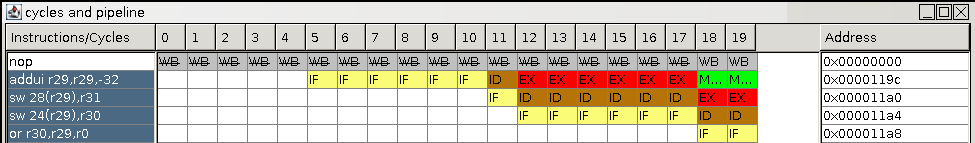
\includegraphics[width=\textwidth-2cm]{images/pipeline_forwarding.png}
\end{center}

There are such unfinished instructions in the following screenshot :

\begin{center}
	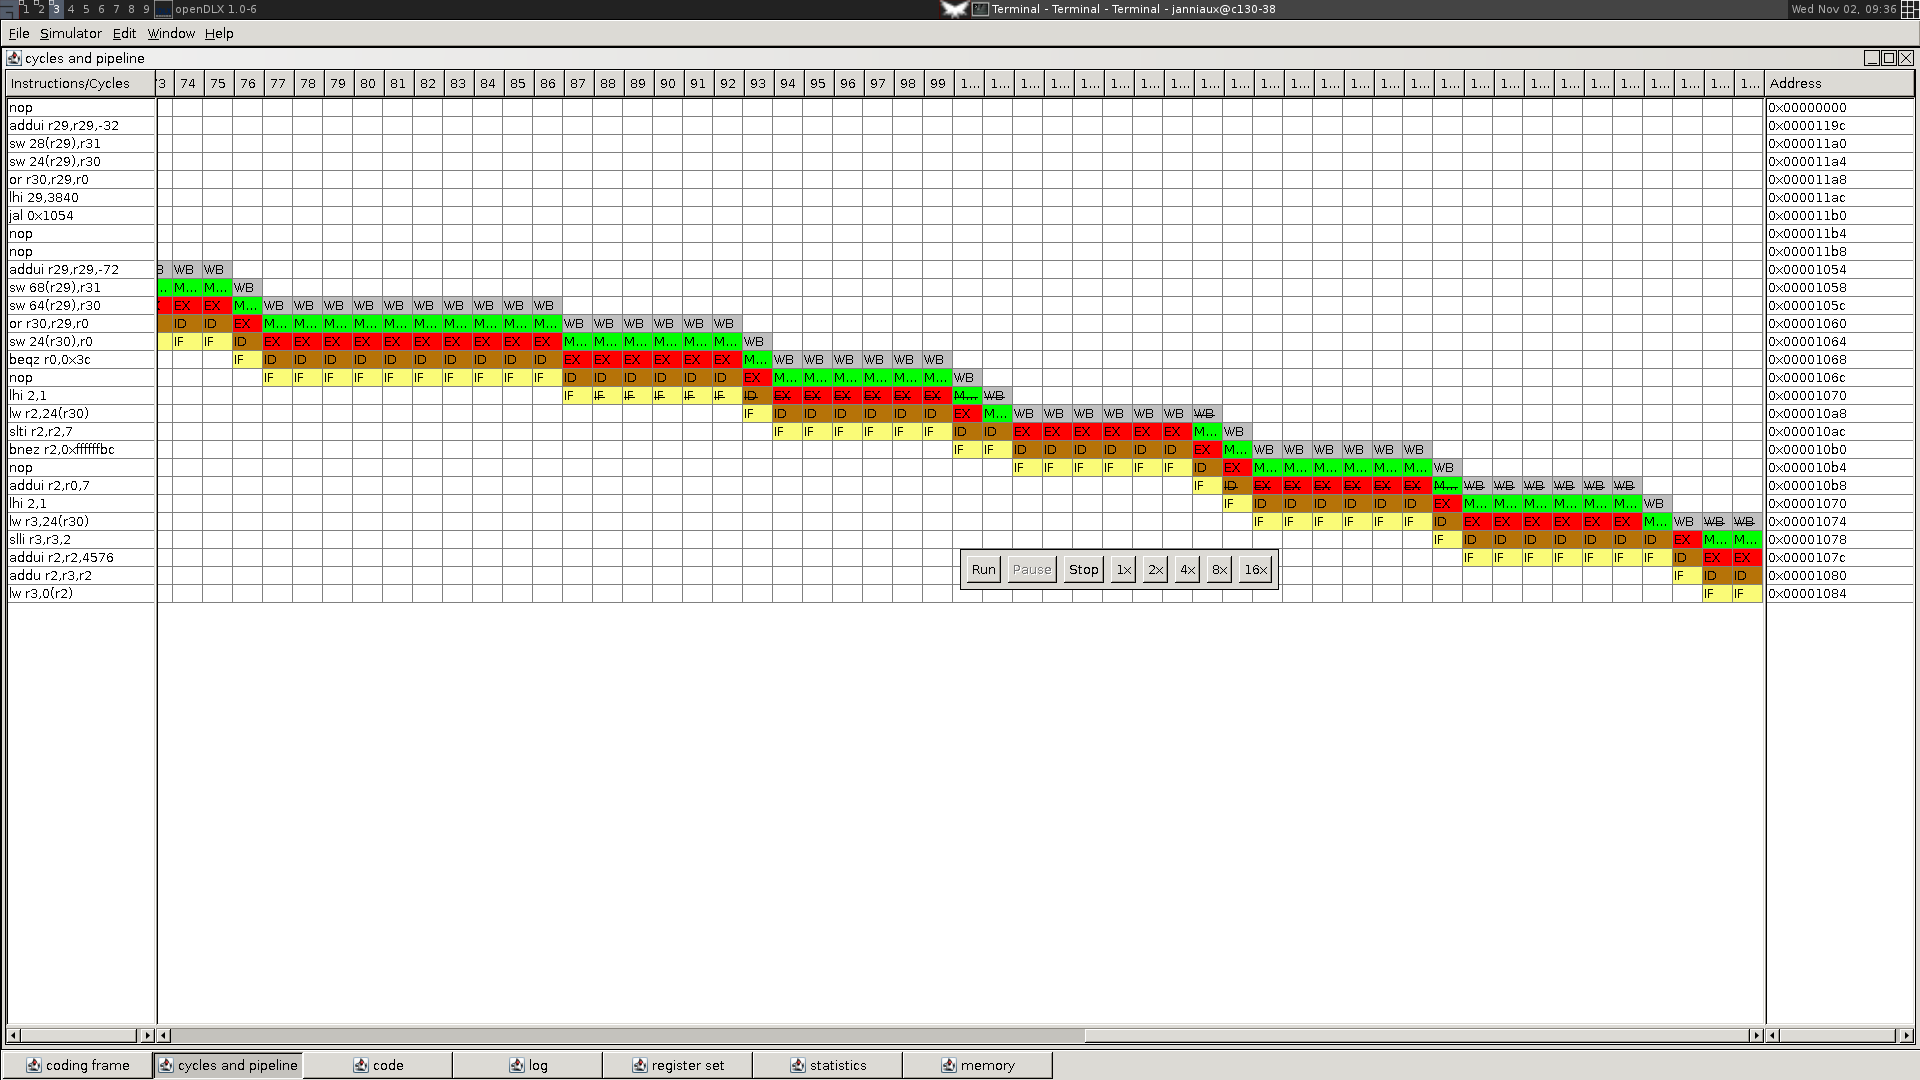
\includegraphics[width=\textwidth-2cm]{images/pipeline_no_writeback_after_branching.png}
\end{center}

Here we can see that the \texttt{lhi 2,1} instruction never reaches the WB stage. This is because the
\texttt{beqz~r0,0x3c} was mispredicted, thus the instruction is flushed, discarding its result.

\begin{center}
	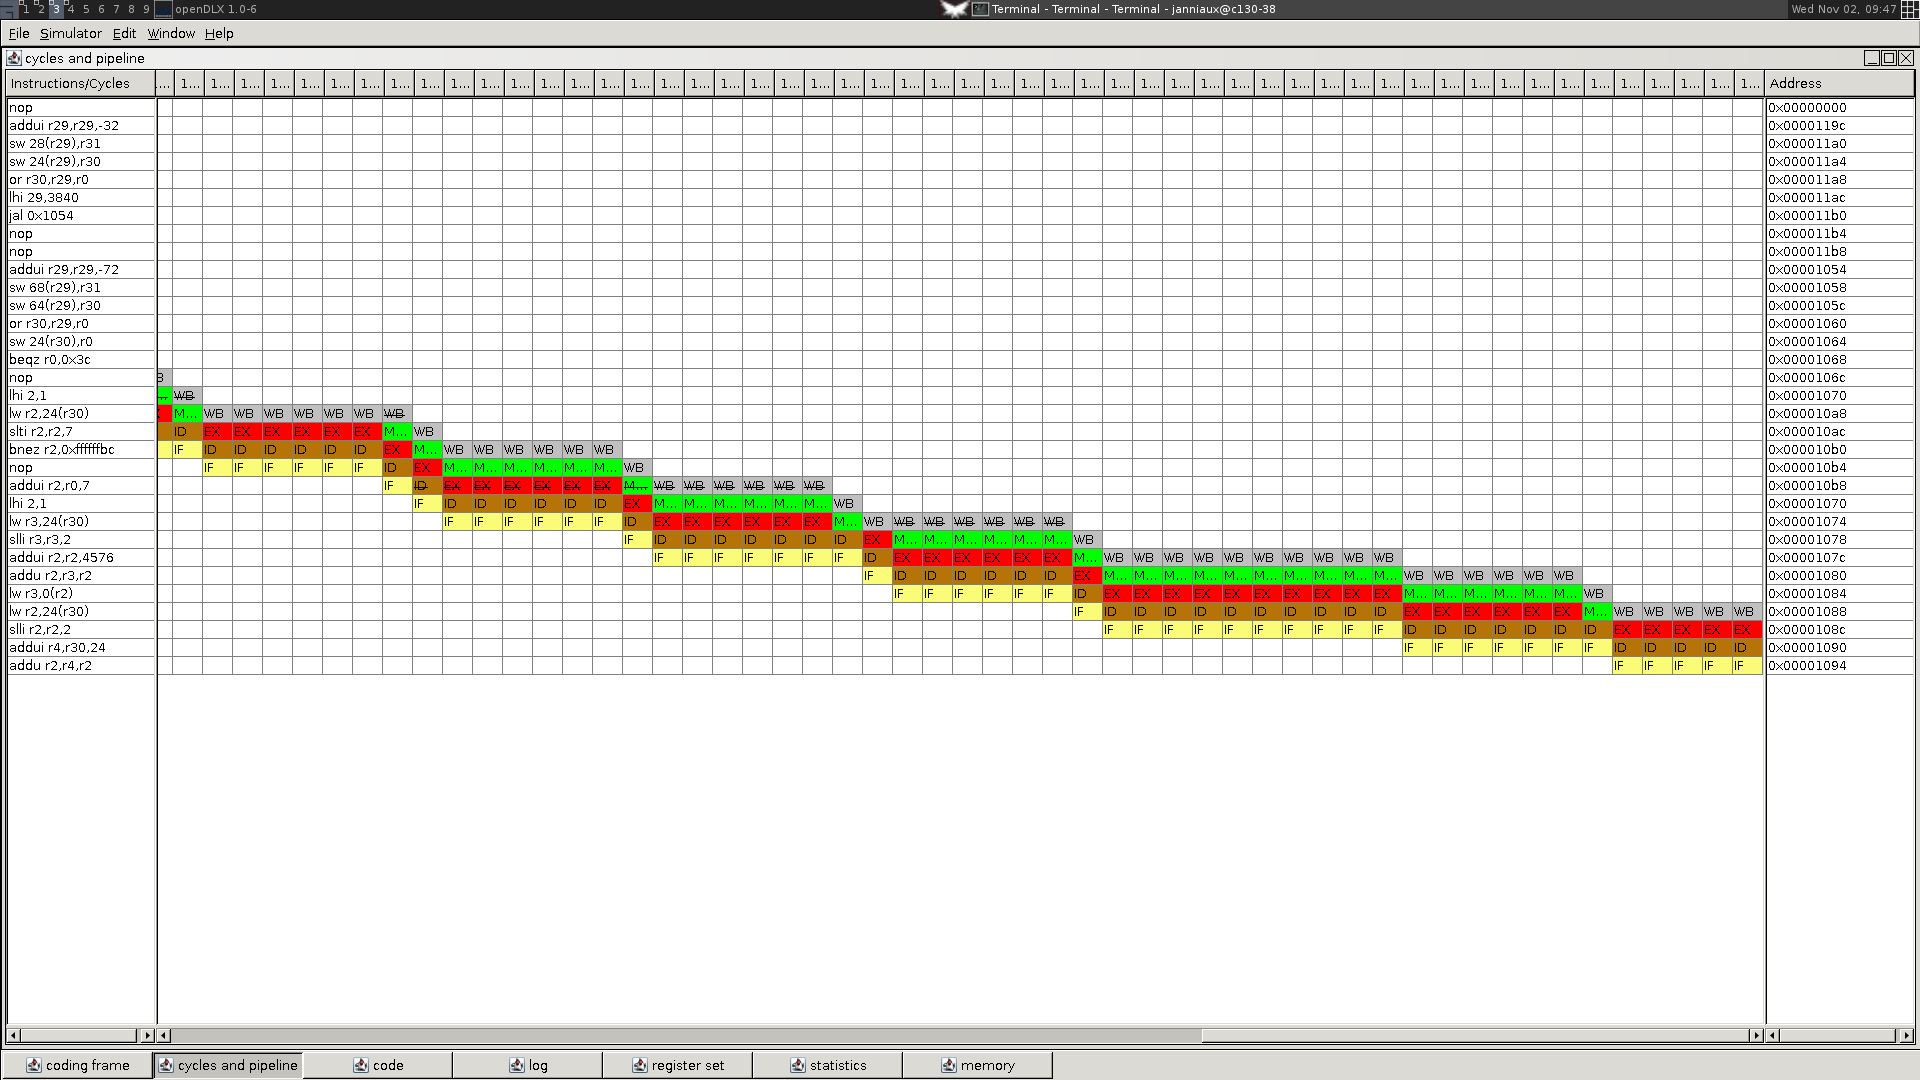
\includegraphics[width=\textwidth-2cm]{images/pipeline_no_writeback_after_forwarding.png}
\end{center}

In this part, we see that the \texttt{lw~r3,24(r30)} is not written back to the registers because its output
register, \texttt{r3}, is reused by the next instruction as an input and an output. Thus the value stays in
the pipeline because it is forwarded, it would be erased otherwise.
\mbox{}\\

Overall we notice that all branches are handled the same way : branch instructions are followed by a
\texttt{nop} that is fully executed, then by another instruction that is discarded (flushed). This is because
the branch predictor needs a full cycle to tell wether it mispredicted.

\section{Branch prediction}

1-bit Branch Predictor :
\begin{verbatim}
Cycles: 3908
Executed instructions: 2788
Performed fetches: 2503
Jumps correctly predicted: 169 mispredicted: 40 misprediction rate: 19,14%
\end{verbatim}
2-bit Branch Predictor
\begin{verbatim}
Cycles: 3904
Executed instructions: 2788
Performed fetches: 2499
Jumps correctly predicted: 163 mispredicted: 36 misprediction rate: 18,09%
\end{verbatim}

Overall, the 2-bit predictor saved us 4 cycles over the 1-bit predictor and lowered the misprediction rate
from 19,14\% to 18,09\%. Although the benefits look small, they are instresting as a 2-bit saturation
predictor is rather simple logic.

It is important to note that, following an update of openDLX, the total jump count is lower in the 2-bit
simulation than in the 1-bit one.
\mbox{}\\

\noindent 1-bit Branch Predictor :
\begin{verbatim}
bpc: 0x0000104c [76] tgts: [0x0000113c] a:66 t/nt: 66/0 mp/cp: 5/61 mp-ratio: 0,08
bpc: 0x00001104 [4] tgts: [0x0000113c] a:56 t/nt: 10/46 mp/cp: 9/47 mp-ratio: 0,16
bpc: 0x00001158 [88] tgts: [0x000010d4] a:27 t/nt: 21/6 mp/cp: 12/15 mp-ratio: 0,44
bpc: 0x00001134 [52] tgts: [0x00001000] a:16 t/nt: 16/0 mp/cp: 1/15 mp-ratio: 0,06
bpc: 0x000010cc [76] tgts: [0x00001148] a:11 t/nt: 11/0 mp/cp: 6/5 mp-ratio: 0,55
bpc: 0x000010b0 [48] tgts: [0x00001070] a:8 t/nt: 7/1 mp/cp: 2/6 mp-ratio: 0,25
bpc: 0x00001174 [116] tgts: [0x000010c8] a:7 t/nt: 6/1 mp/cp: 2/5 mp-ratio: 0,29
bpc: 0x00001068 [104] tgts: [0x000010a8] a:6 t/nt: 6/0 mp/cp: 1/5 mp-ratio: 0,17
bpc: 0x000010c0 [64] tgts: [0x0000116c] a:6 t/nt: 6/0 mp/cp: 1/5 mp-ratio: 0,17
bpc: 0x000011b0 [48] tgts: [0x00001054] a:6 t/nt: 6/0 mp/cp: 1/5 mp-ratio: 0,17
\end{verbatim}
2-bit Branch Predictor :
\begin{verbatim}
bpc: 0x0000104c [76] tgts: [0x0000113c] a:66 t/nt: 66/0 mp/cp: 5/61 mp-ratio: 0,08
bpc: 0x00001104 [4] tgts: [0x0000113c] a:46 t/nt: 10/36 mp/cp: 10/36 mp-ratio: 0,22
bpc: 0x00001158 [88] tgts: [0x000010d4] a:27 t/nt: 21/6 mp/cp: 7/20 mp-ratio: 0,26
bpc: 0x00001134 [52] tgts: [0x00001000] a:16 t/nt: 16/0 mp/cp: 1/15 mp-ratio: 0,06
bpc: 0x000010cc [76] tgts: [0x00001148] a:11 t/nt: 11/0 mp/cp: 6/5 mp-ratio: 0,55
bpc: 0x000010b0 [48] tgts: [0x00001070] a:8 t/nt: 7/1 mp/cp: 2/6 mp-ratio: 0,25
bpc: 0x00001174 [116] tgts: [0x000010c8] a:7 t/nt: 6/1 mp/cp: 2/5 mp-ratio: 0,29
bpc: 0x00001068 [104] tgts: [0x000010a8] a:6 t/nt: 6/0 mp/cp: 1/5 mp-ratio: 0,17
bpc: 0x000010c0 [64] tgts: [0x0000116c] a:6 t/nt: 6/0 mp/cp: 1/5 mp-ratio: 0,17
bpc: 0x000011b0 [48] tgts: [0x00001054] a:6 t/nt: 6/0 mp/cp: 1/5 mp-ratio: 0,17
\end{verbatim}

Only lines 2 and 3 do differ between the 1-bit and the 2-bit BPC. Although the second branch is a bit worse
with a misprediction rate of 0,22 compared to the ratio of 0,16 (37.5\% worsening) of the 1-bit BPC, the third
branch is ways better with a rate of 0,26 instead of 0,44 (59\% improvement). Overall, the 2-bit BPC is
better.

% TODO

\section{Data Caches}

\begin{verbatim}
Dcache: used rpol: DIRECT_MAPPED wpol: WRITE_THROUGH lines: 4 associativity: 1
    line_size: 4 total size: 16
Accesses: 488 hits: 364 misses: 124 hit rate: 74,59% loaded words: 124
\end{verbatim}

We see that over 488 accesses, 364 were hits while 124 were misses, leading to a hit rate of 74,59\%. The
total cache size is 16.
\mbox{}\\

When we change the line count of the cache, we observe the following results :

\begin{center}
	\begin{tabular}{|r||c|c|c|c|c|}
		\hline
		Line count & 4 & 8 & 16 & 32 & 64 \\
		Cache size & 16 & 32 & 64 & 128 & 256 \\
		Misses     & 124 & 56 & 15 & 7 & 7 \\
		Hit rate   & 74,59\% & 90,86\% & 97,82\% & 99,04\% & 99,04\% \\
		\hline
	\end{tabular}
\end{center}

The best configuration seems to be the 32-line cache since it minimizes the miss count to the absolute minimum
of cache misses, needed for the first ever fetch (compulsory misses).
\mbox{}\\

By changing the associativity parameter, we gain the following results :

\begin{center}
	\begin{tabular}{|c|r||c|c|c|}
		\hline
		\multicolumn{2}{|c||}{Associativity} & 2 & 4 & 8 \\
		\hline
		\multirow{2}{*}{Misses}   & FIFO  & 50 & 44 & 47 \\
		                          & LRU   & 52 & 47 & 80 \\
		\multirow{2}{*}{Hit rate} & FIFO  & 91,78\% & 93,36\% & 92,69\% \\
		                          & LRU   & 91.23\% & 92,52\% & 84,10\% \\
		\hline
	\end{tabular}
\end{center}

By switching the replacement policies to FIFO and setting the associativity to 4, we can increase the hit
rate from 90,86\% (8 lines) to 93,36\% with the same cache size of 32.

\end{document}


